\documentclass[a4paper, 11pt]{article}

\usepackage{amsmath}
\usepackage{amssymb}
\usepackage{hyperref}
\usepackage{makeidx}
\usepackage{graphicx}
\graphicspath{{figures/}} % Directory in which figures are stored
\usepackage{natbib}% \bibliography
\usepackage{float}
\usepackage{setspace} % for line spacing
\usepackage[margin=1in]{geometry}
\title{Assignment1-CSE780}
\author{Paria, Fakhrzad \\ Stuent ID: 400353290 }
\date{23-September-2021}
\setstretch{1.5}

\begin{document}

\maketitle
\newpage
\section*{1.Handling missing values}
\subsection*{Part a:  before cleansing and tidying}
 We used NOAA*GSOD dataset that is related to measuring climate features(27 variabe) with station and recorded-time as keys~\cite{ref}.lets plot the histogram across 10000 records in figure\ref{Figure1a} for "visib"and"gust". It seems the data needs to be tidy.
\subsection*{Part b : doing cleansing}
We use formula of filtering for removing samples that are out of range.Out of 10000 records It just extracted 2271 clean ones.
\subsection*{Part c : after tidying}
The plotted Histogram after tidying in figure2 shows the worst visible times have recorded in the bigger gust.
 \begin{figure}[H]
	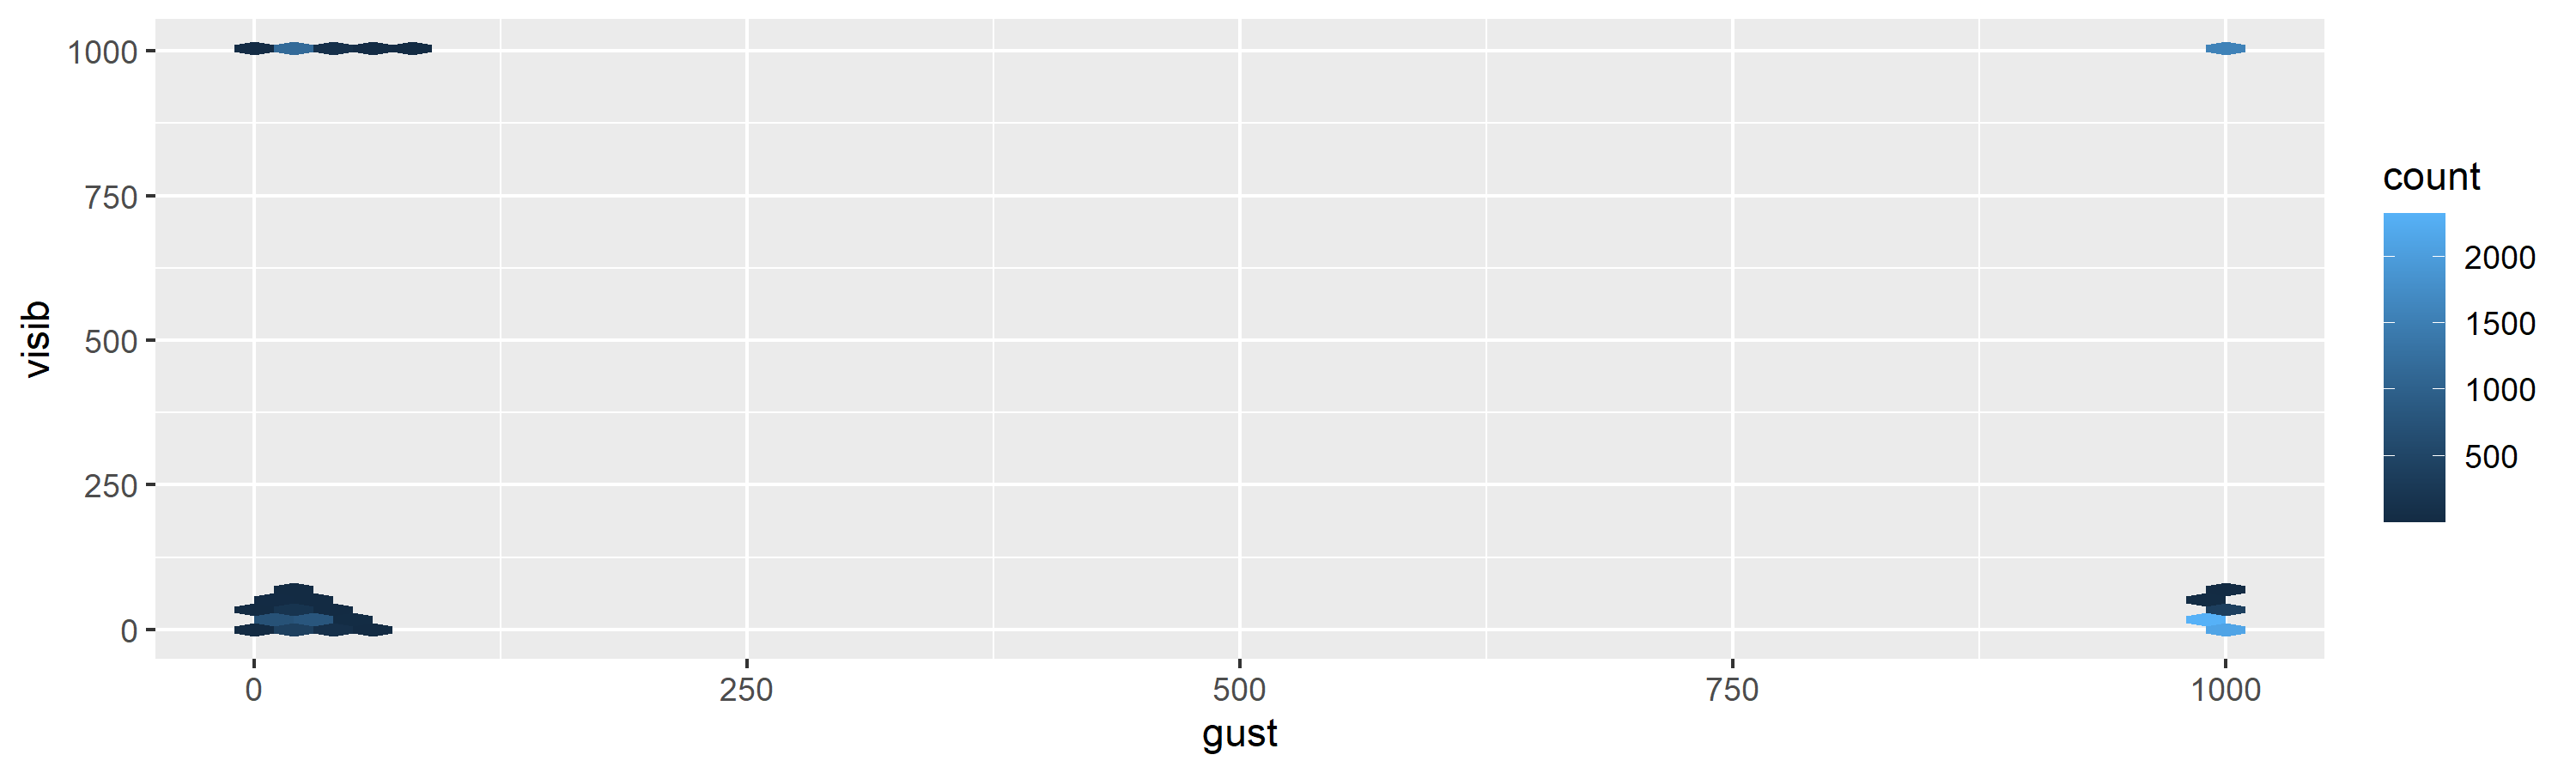
\includegraphics[width = \textwidth]{figure1a.png}
	\caption{Histogram of visib and gust.}
	\label{Figure1a}
\end{figure}
 \begin{figure}[H]
	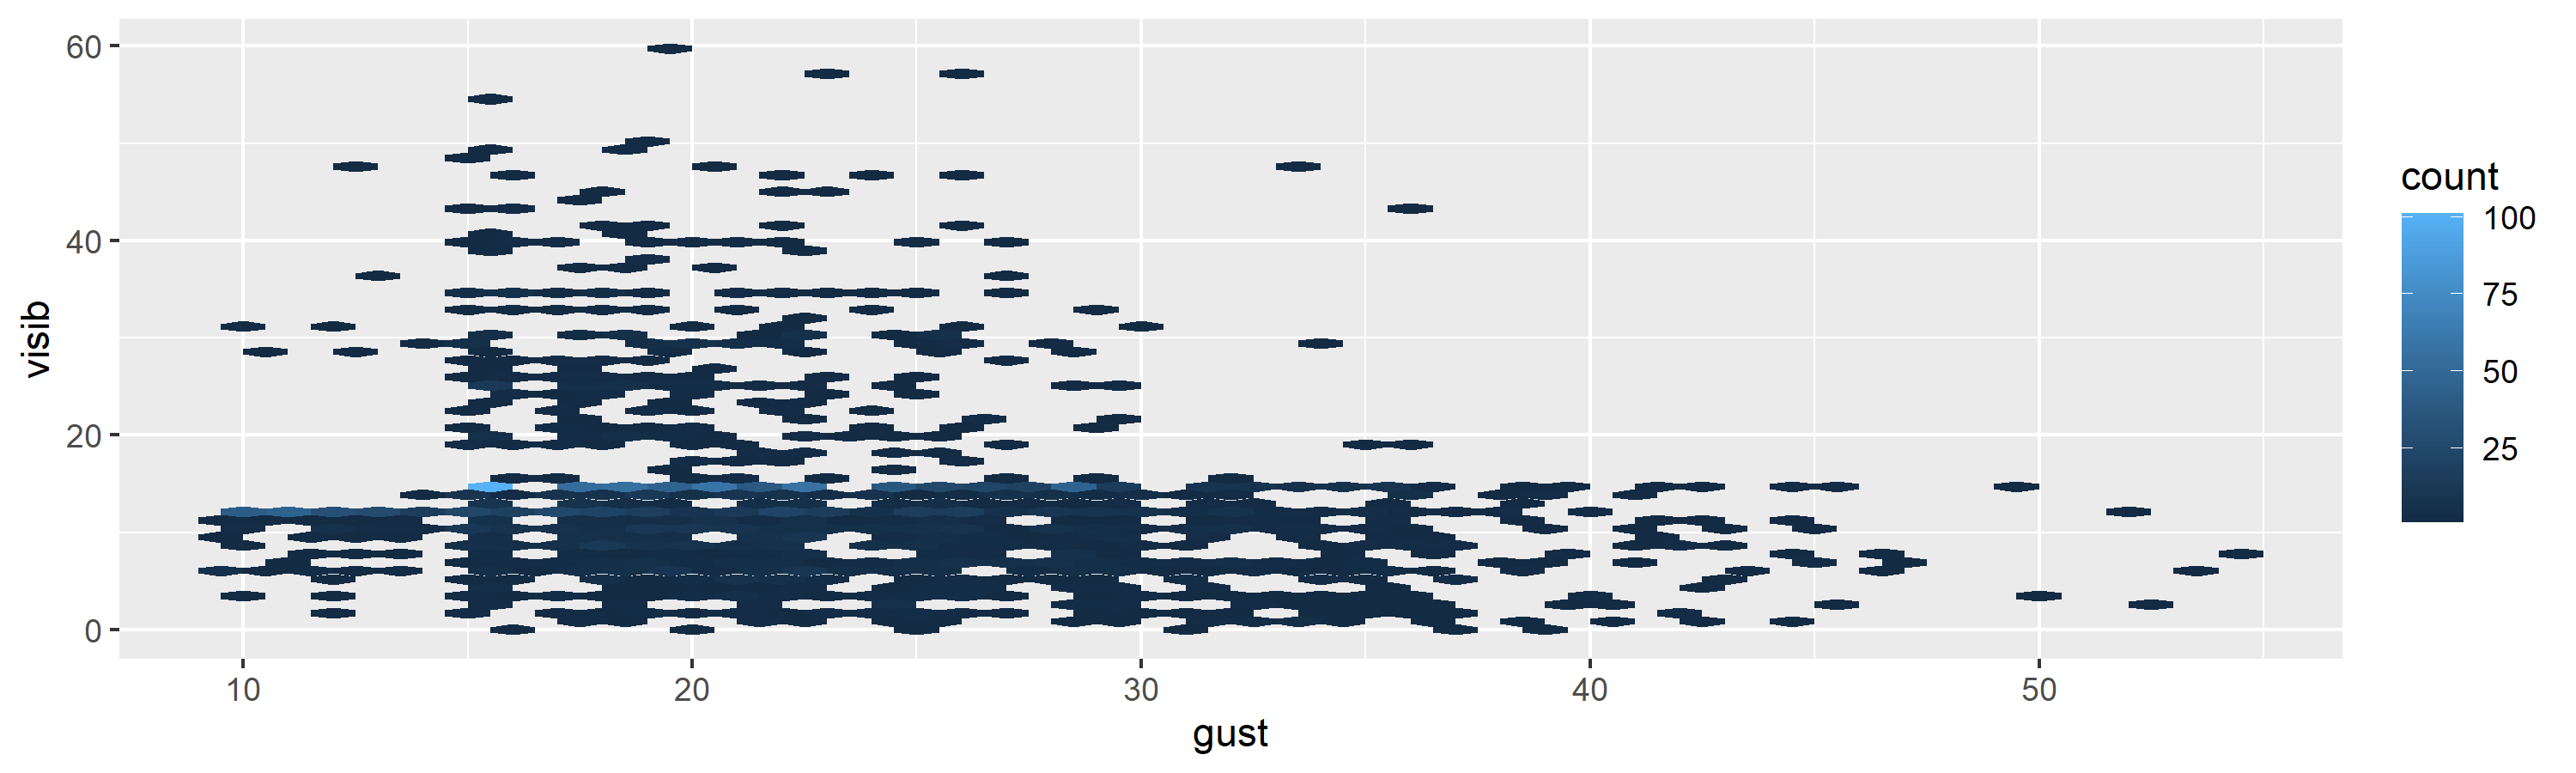
\includegraphics[width = \textwidth]{figure1b.png}
	\caption{Histogram of visib and gust after tidying.}
	\label{Figure1b}
\end{figure}


\newpage
\section*{2.Making a heatmap}
\subsection*{2.a: using the raw data}
In this section we plot a heatmap to shows gene expression after the first symmetry breaking event of the embryo. Since the number of genes are huge there is no clear clue to find the relationships visually[figure2a]

\subsection*{2.b: Clustering data}
With aid of determining 10 clusters in gene, \cite{pheatmap} we can see that some samples have the most proportion of measure in interval -2 and -4.[figure2b]

\begin{figure}[H]
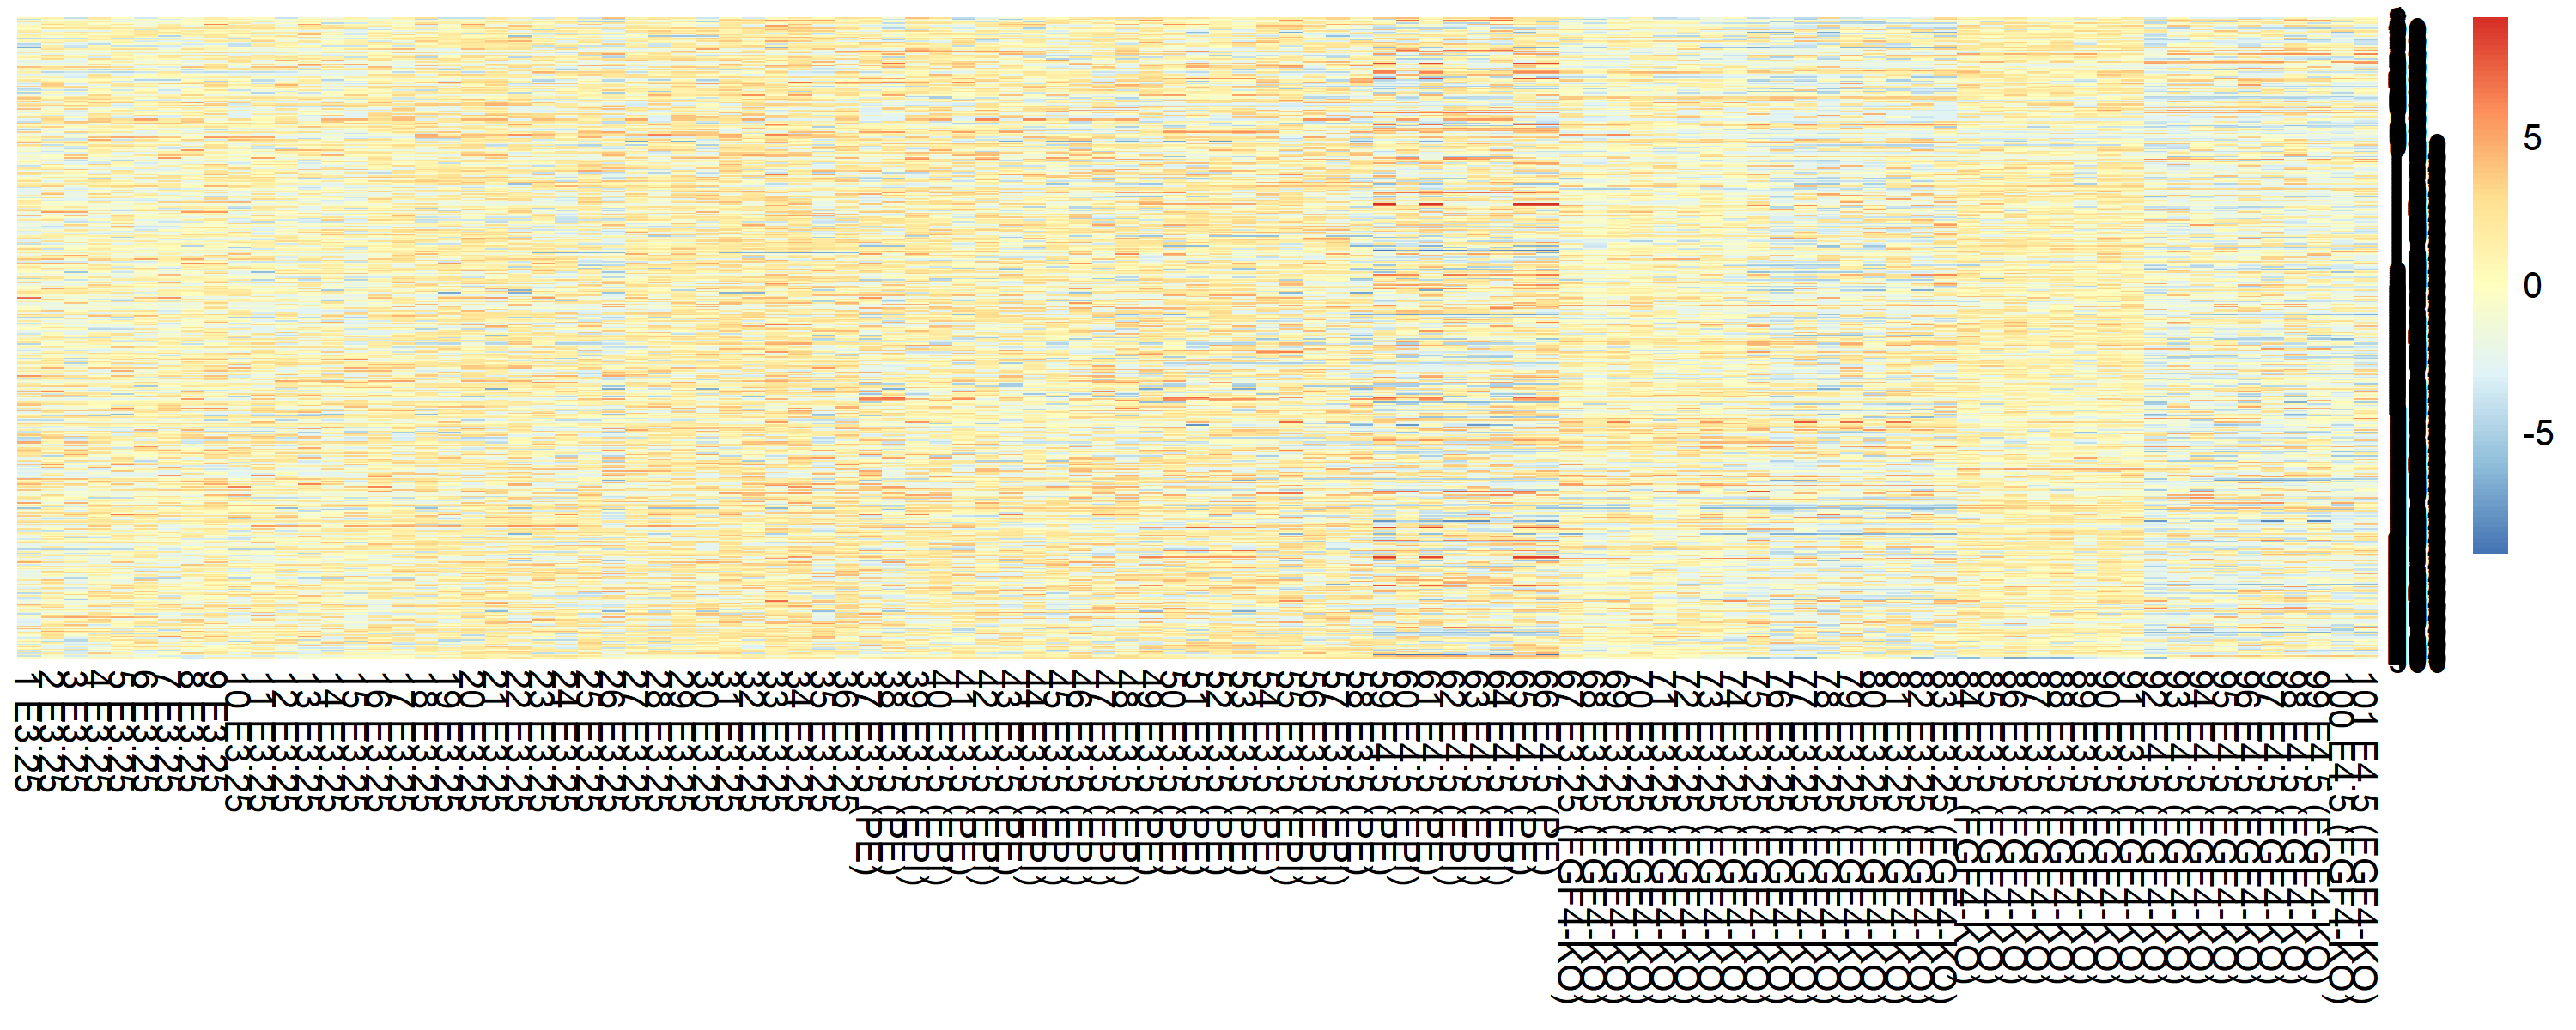
\includegraphics[width = \textwidth]{figure2a.png}
\caption{heatmap of gene and embryo's symmetry breaking samples .}
\label{Figure2a}
\end{figure}
\begin{figure}[H]
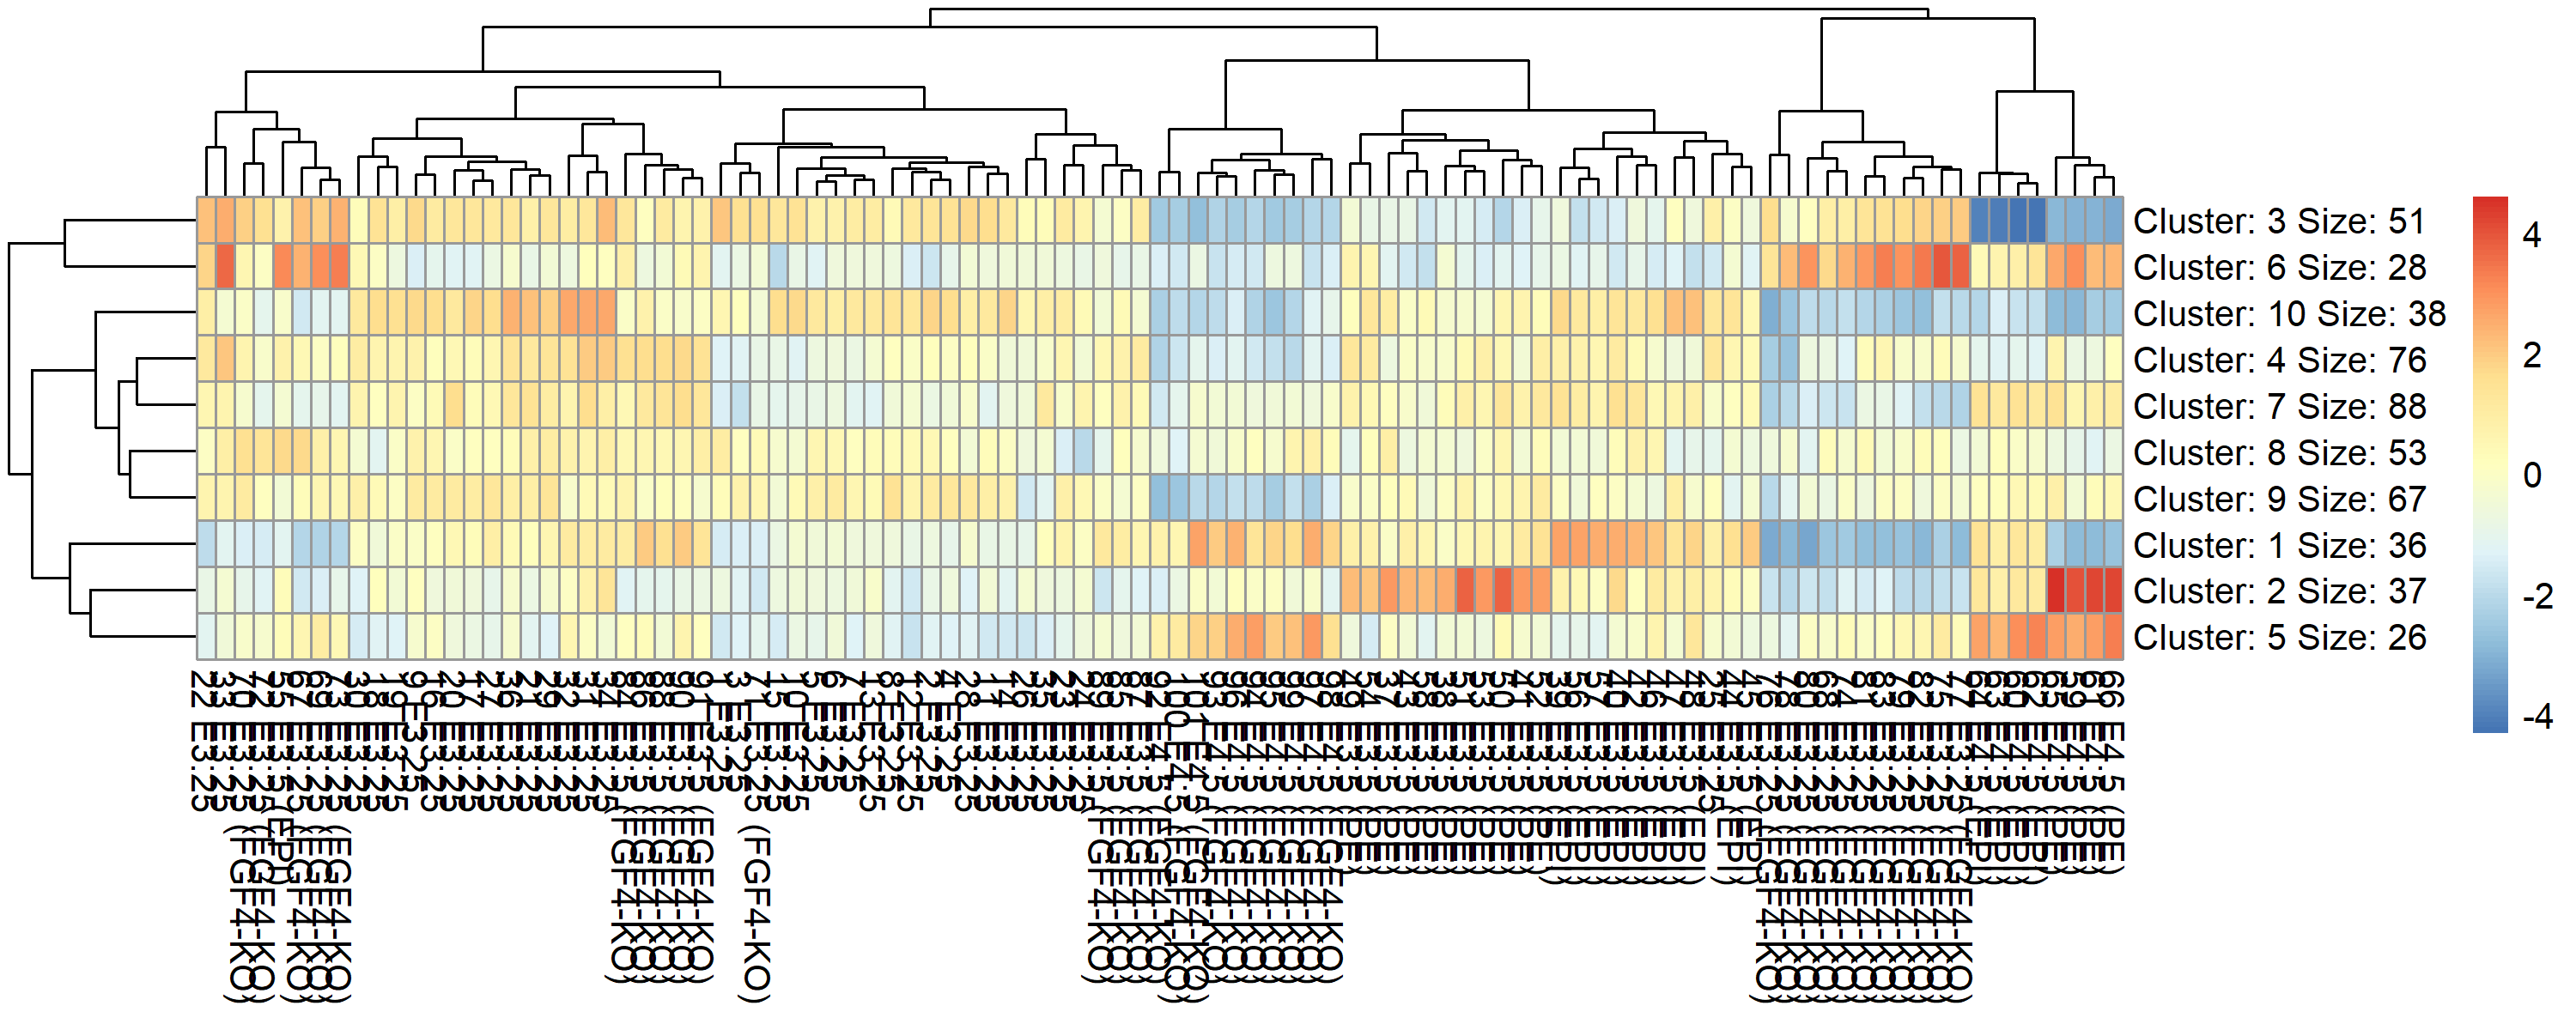
\includegraphics[width = \textwidth]{figure2b.png}
\caption{Clustered heatmap.}
\label{Figure2b}
\end{figure}

\newpage
\section*{3. having a dataset analysis}
\subsection*{3.a: Describe data}
The data that has been used in this section is related to supply chain records in 4 years.~\cite{scm}

\subsection*{3.b: Summary of data}
Table1 shows the summary of data in the table \ref{sumInfo}.
\begin{table}[H]
	\centering
	\caption{Summary of used SCM characters}
	\label{sumInfo}
	\begin{tabular}{|c|c|c|c|c|c|c|}
		\hline
		\textbf{Variable} & \textbf{count} &  \textbf{type} &  \textbf{min} &  \textbf{max} &  \textbf{mean} &  \textbf{null} \\
		\hline		
		Shipping days & 1:180519 & num & 0 & 6 & 3.498 & 0\\
		Type & 1:180519 & chr &  &  &  & \\
		discount rate & 1:180519 & num & 0 & 0.25 & 0.1 & 0\\
		order date & 1:180519 & chr &  &  &  & 0\\
		shipment date & 1:180519 & chr &  &  &  & 0\\
		shipment class & 1:180519 & chr &  &  &  & 0\\
		product group & 1:180519 & chr &  &  &  & 0\\
		\hline 
	\end{tabular}
\end{table}


\subsection*{3.c: Visualizing the data}
In figure5 we plot the trend of number of orders in four years categorized per delivery status. It is clear that portion of late deliver is more than other parts.
In figure6 red points are the late shipment that in some regions are more than others also most of shipment days more than 4days caused late delivery.
In figure7 despite the nature of priority classes it shows that the proportion of delayed delivery in first class orders is undeniably more that other categories. 

\subsection*{3.d: Making a shiny app}
There is a app that you can use to find in each product category how many orders we had in these four years and what was the order status( on time or delayed).
the link of this app is : \url{https://vmbe7g-paria-fakhrzad.shinyapps.io/Smart_Supply_chain/}


\begin{figure}[H]
	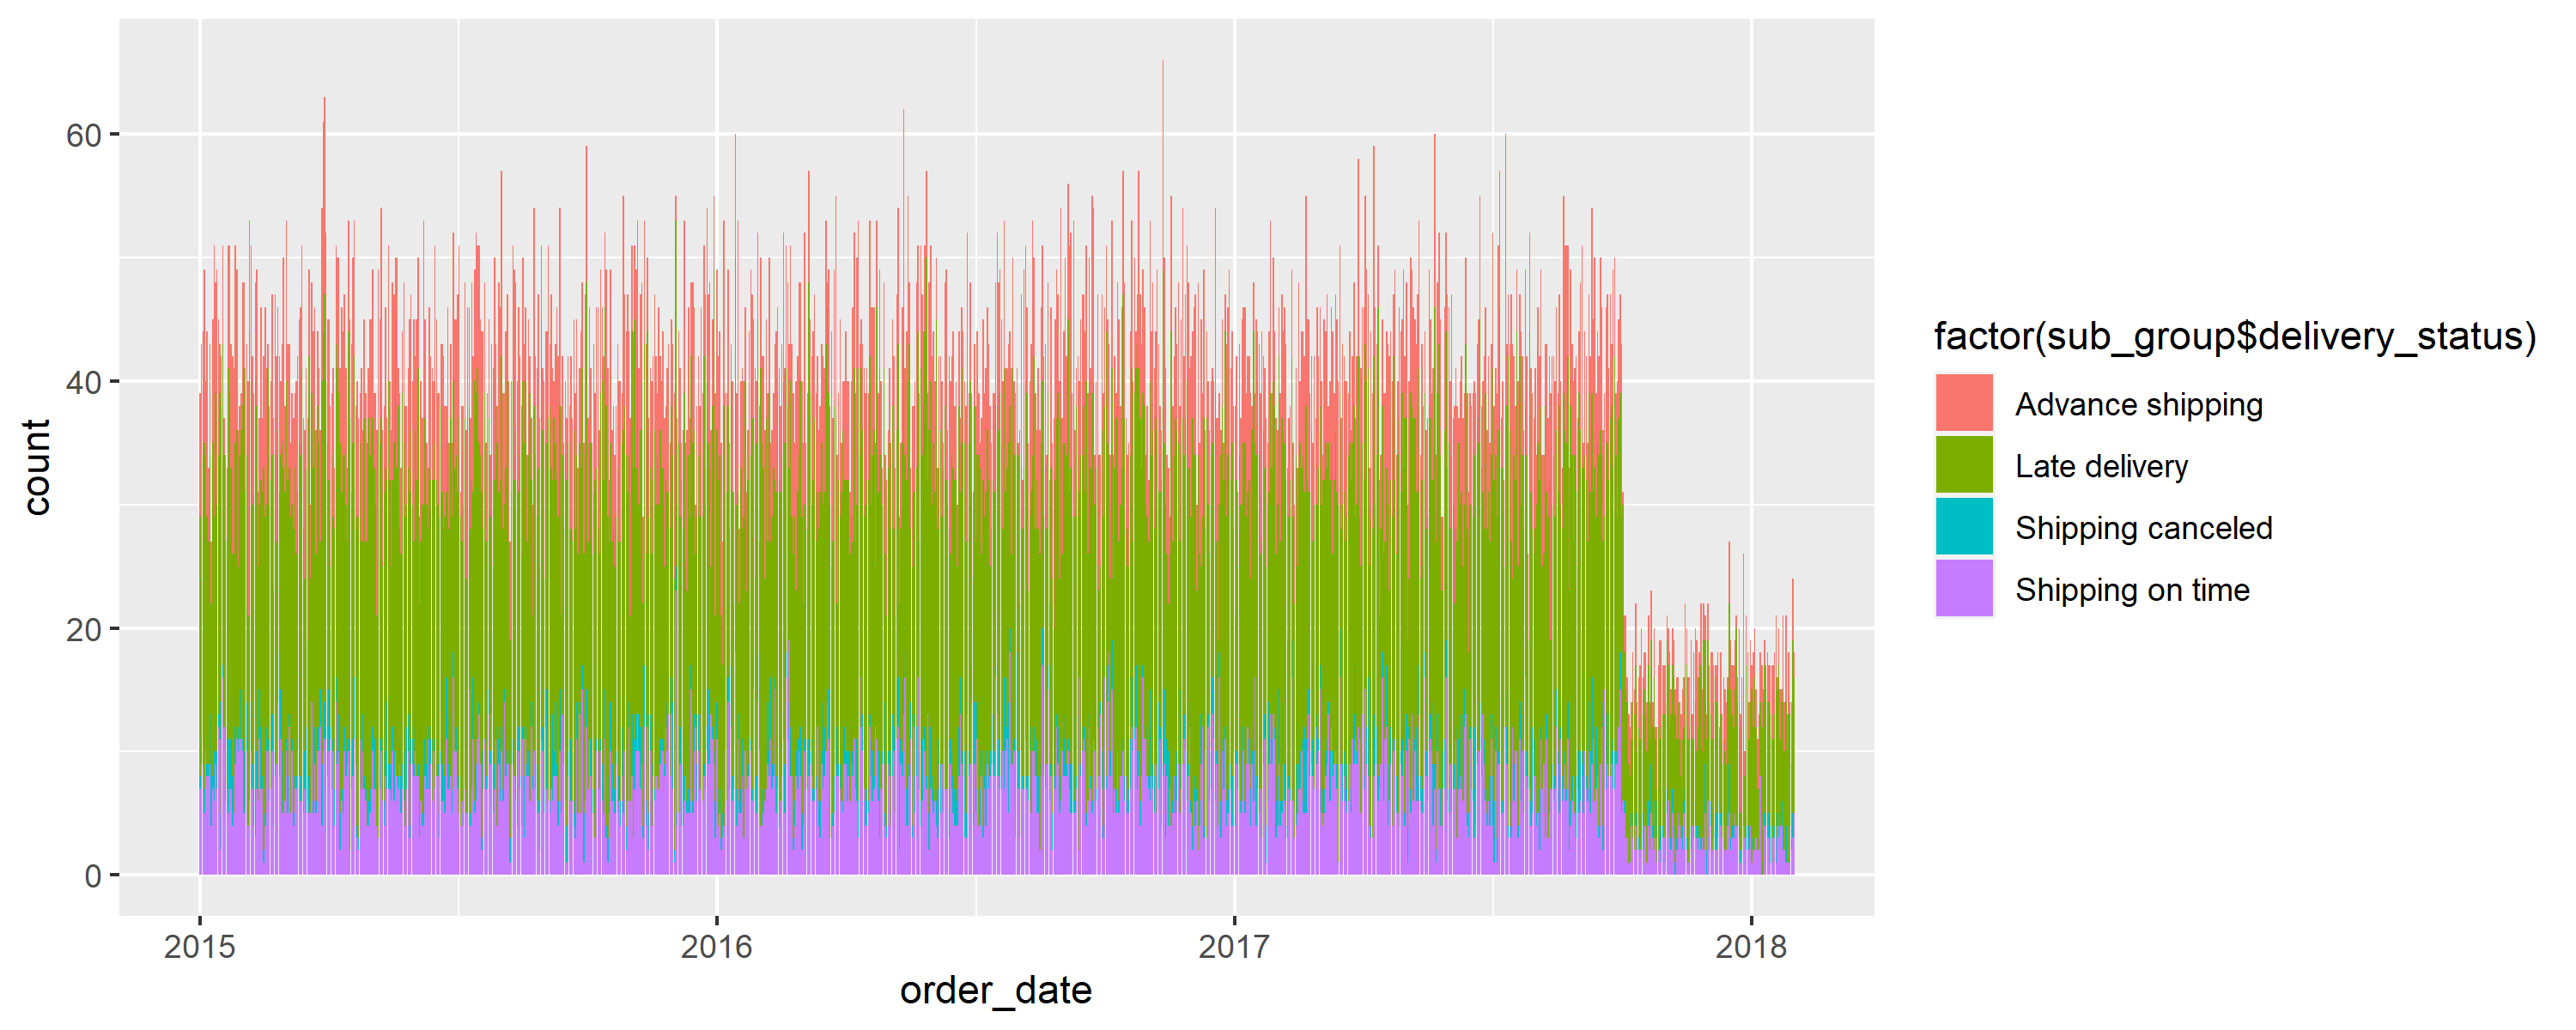
\includegraphics[width = \textwidth]{figure3a.png}
	\caption{order date trend colored by delivery status}
	\label{Figure3a}
\end{figure}
\begin{figure}[H]
	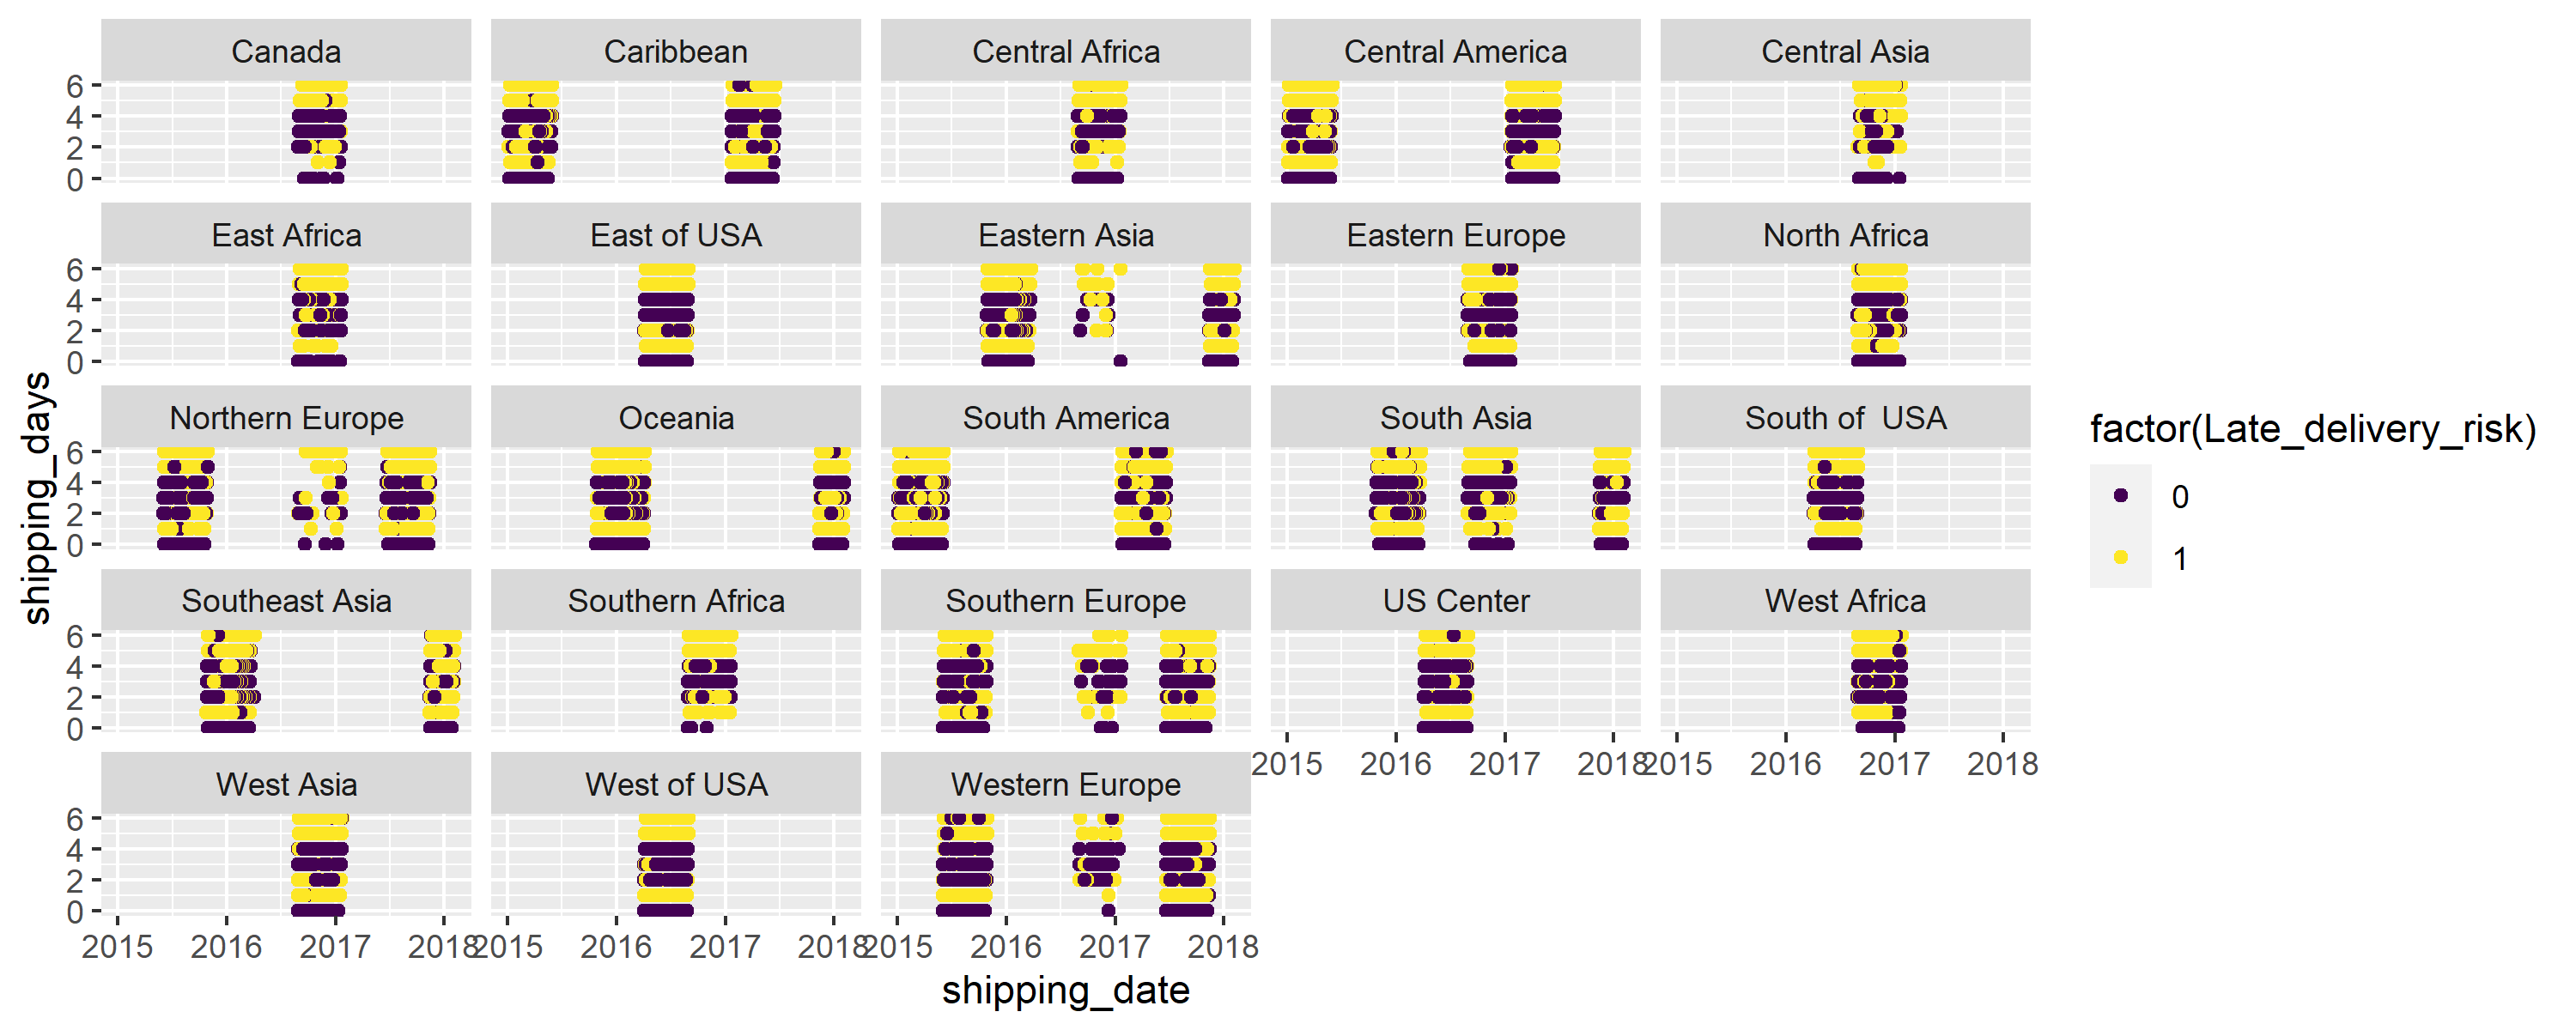
\includegraphics[width = \textwidth]{figure3b.png}
	\caption{late delivery status by region}
	\label{Figure3b}
\end{figure}
\begin{figure}[H]
	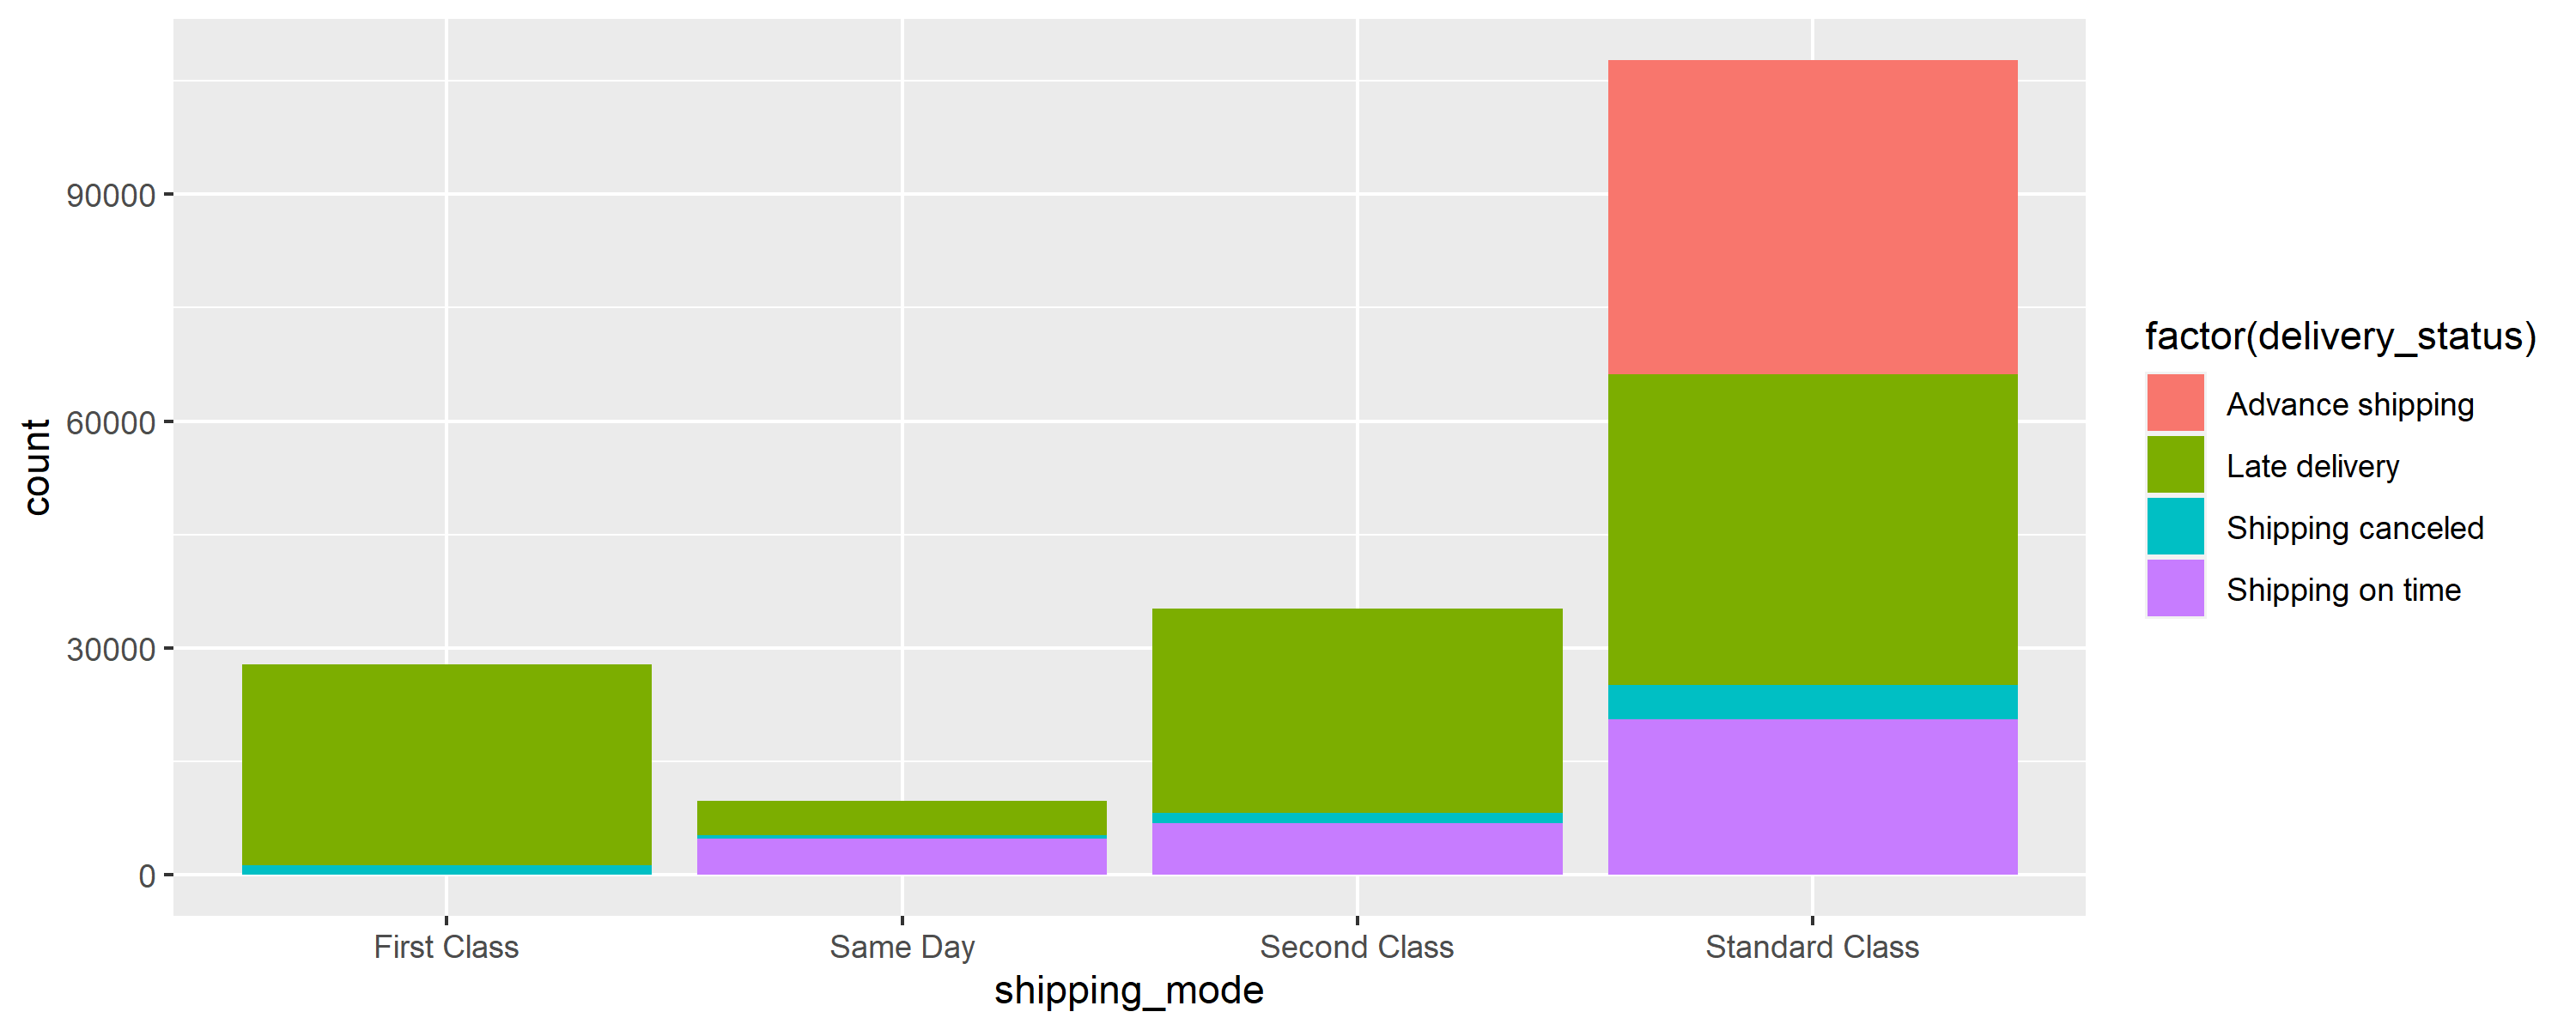
\includegraphics[width = \textwidth]{figure3c.png}
	\caption{profit vs discount}
	\label{Figure3c}
\end{figure}


\newpage
\bibliographystyle{apa}
\bibliography{Assignment1}

\end{document}
